\documentclass{standalone}
\usepackage{tikz}


\begin{document}

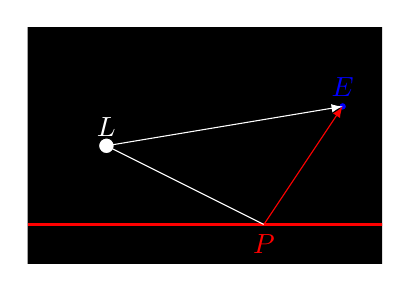
\begin{tikzpicture}
  \path[clip] (-1,-0.5) rectangle (3.5,2.5);
  \draw[fill=black,black] (-1,-0.5) rectangle (3.5,2.5);
  \draw[thick,red] (-1,0) -- (4,0);

  \coordinate (light) at (0,1);
  \coordinate (hit) at (2,0);
  \coordinate (eye) at (3,1.5);
  
  \draw[fill=blue] (eye) circle [radius=0.05cm] node[above,blue] {$E$};
  \draw[fill=white] (light) circle [radius=0.1cm] node [white,above] {$L$};
  \node[anchor=north,red] at (hit) {$P$};
  \draw[white] (light) -- (hit);
  \draw[white,-latex] (light) -- (eye);
  \draw[red,-latex] (hit) -- (eye);
\end{tikzpicture}

\end{document}